\section{Formal Grammars}

Now we introduce formal grammars as a way of building up our language.
This is similar to English, where we have a grammar system that tells us how to build sentences.
For example, we know the basic structure of a sentence is \textit{subject-verb-object}. \\

\noindent
We can write \textbf{linear} statements such as ``John hit the ball'', which has an underlying \textbf{hierarchical} structure that permits it:

\begin{figure}[h]
\centering
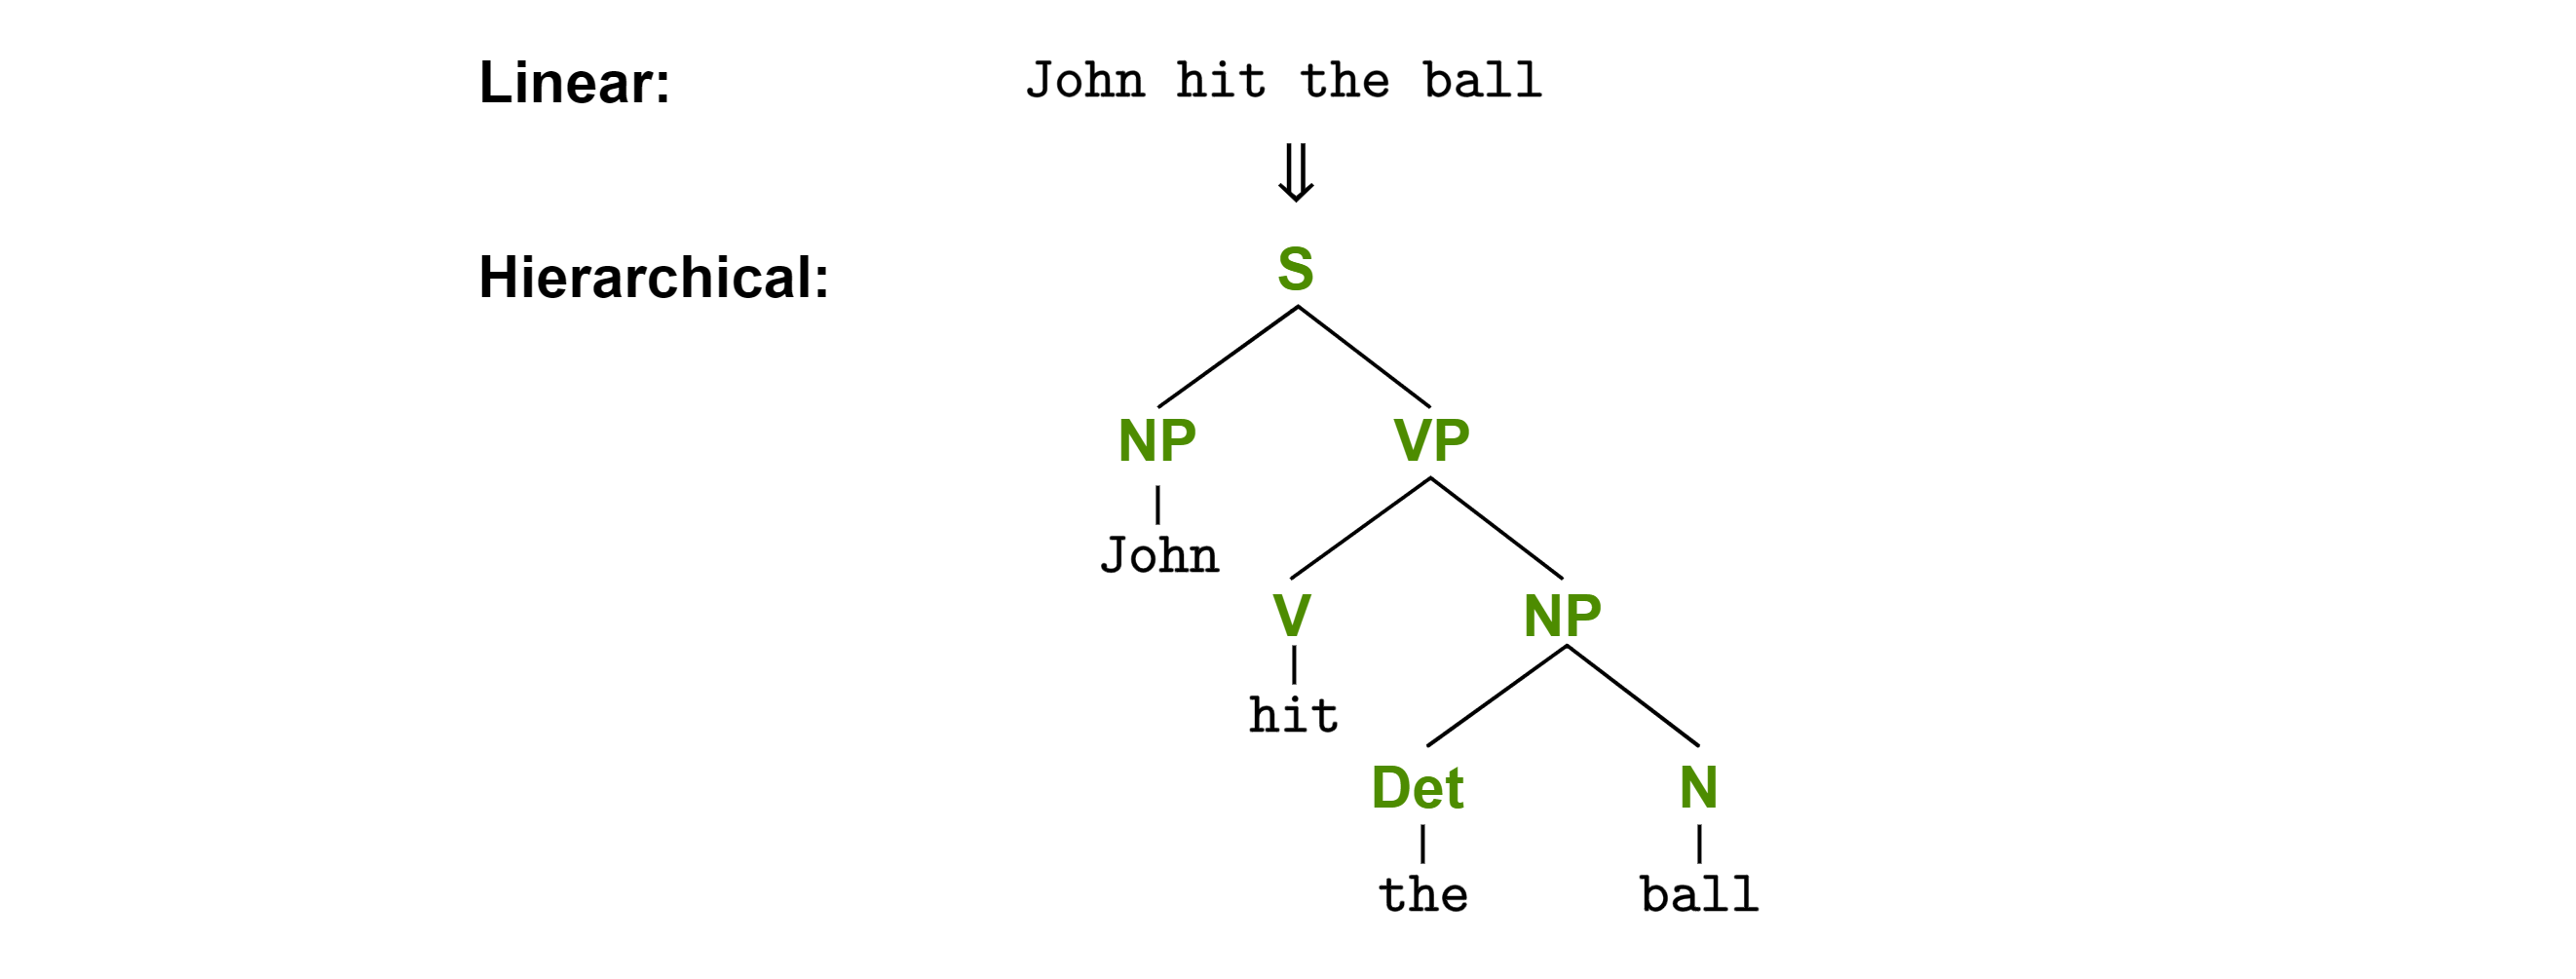
\includegraphics[width=1\textwidth]{Sections/Formal/eng.png}
\caption{The sentence ``John hit the ball'' has an underlying hierarchical structure of a tree. Here, \textbf{S}: Sentence (the root of the tree), \textbf{NP}: Noun Phrase (a phrase centered around a noun), \textbf{VP}: Verb Phrase (a phrase centered around a verb), \textbf{V}: Verb (the action in the sentence), \textbf{Det}: Determiner (words like "the", "a", "an", which specify nouns), and \textbf{N}: Noun (person, place, thing, or idea).}
\end{figure}

\noindent
\textbf{Grammar vs. Semantics:} Notice the english sentence 

\begin{center}
\Large \textit{``Your air tied a toothbrush at school!''}
\end{center}

\noindent
is grammatically correct, but carries little to no meaning. In contrast, 
the sentence

\begin{center}
\Large \textit{``Colorless the of allegator run am sleepily''}
\end{center}

\noindent
is perhaps an unsettling read, as it is not grammatically correct. \\

\newpage 

\noindent
The same way we can represent english sentences in a tree structure, is the same way we can represent programs. First 
we define the difference between an \textbf{interpreter} and a \textbf{compiler}.

\begin{Def}[Interpreter]

    An \textbf{interpreter} is a program that directly executes instructions written in a programming language without 
    requiring a machine code translation. The typical stages are:
    
    \begin{enumerate}
        \item \textbf{Lexical Analysis}: Reads a string of characters (program), converting it into tokens.
        \item \textbf{Syntax Analysis}: Parses these tokens to build an abstract syntax tree (AST).
        \item \textbf{Semantic Analysis}: Checks for semantic errors and annotates the AST.
        \item \textbf{Intermediate Representation (IR) Generation}: Converts the AST into an intermediate representation (IR) to facilitate execution.
        \item \textbf{Direct Execution}: Executes the IR or AST directly using an interpreter.
    \end{enumerate}
    
    \noindent
    Interpreted languages are \textbf{evaluated at runtime} (e.g., Python, Ruby, JavaScript). Some interpreters use an \textbf{AST-based execution}, while others generate an \textbf{IR} (e.g., Python's bytecode for the CPython interpreter).
    
    \end{Def}
    
    \begin{Def}[Compiler]
    
    A \textbf{compiler} is a program that translates code written in a high-level programming language into a lower-level language, typically machine code, to create an executable program. This involves several stages:
    
    \begin{enumerate}
        \item \textbf{Lexical Analysis}: Reads the source code and converts it into tokens.
        \item \textbf{Syntax Analysis}: Parses these tokens to construct an abstract syntax tree (AST).
        \item \textbf{Semantic Analysis}: Validates the AST against language rules and performs type checking.
        \item \textbf{Intermediate Representation (IR) Generation}: Transforms the AST into a lower-level representation that is easier to optimize and translate.
        \item \textbf{Optimization}: Enhances the IR to improve performance and efficiency.
        \item \textbf{Code Generation}: Translates the optimized IR into machine code or another target language.
    \end{enumerate}
    
    \noindent
    Compiled languages are \textbf{translated before runtime} (e.g., C, C++, Rust, OCaml). The \textbf{IR} plays a crucial role in optimizing the compilation process, as seen in LLVM or Java’s bytecode execution in the JVM.
    
    \end{Def}
   
\newpage 

\noindent
The following diagram illustrate the translation process of a compiler and an interpreter:

\vspace{2em}

\begin{figure}[h]
    \hspace{-2em}
    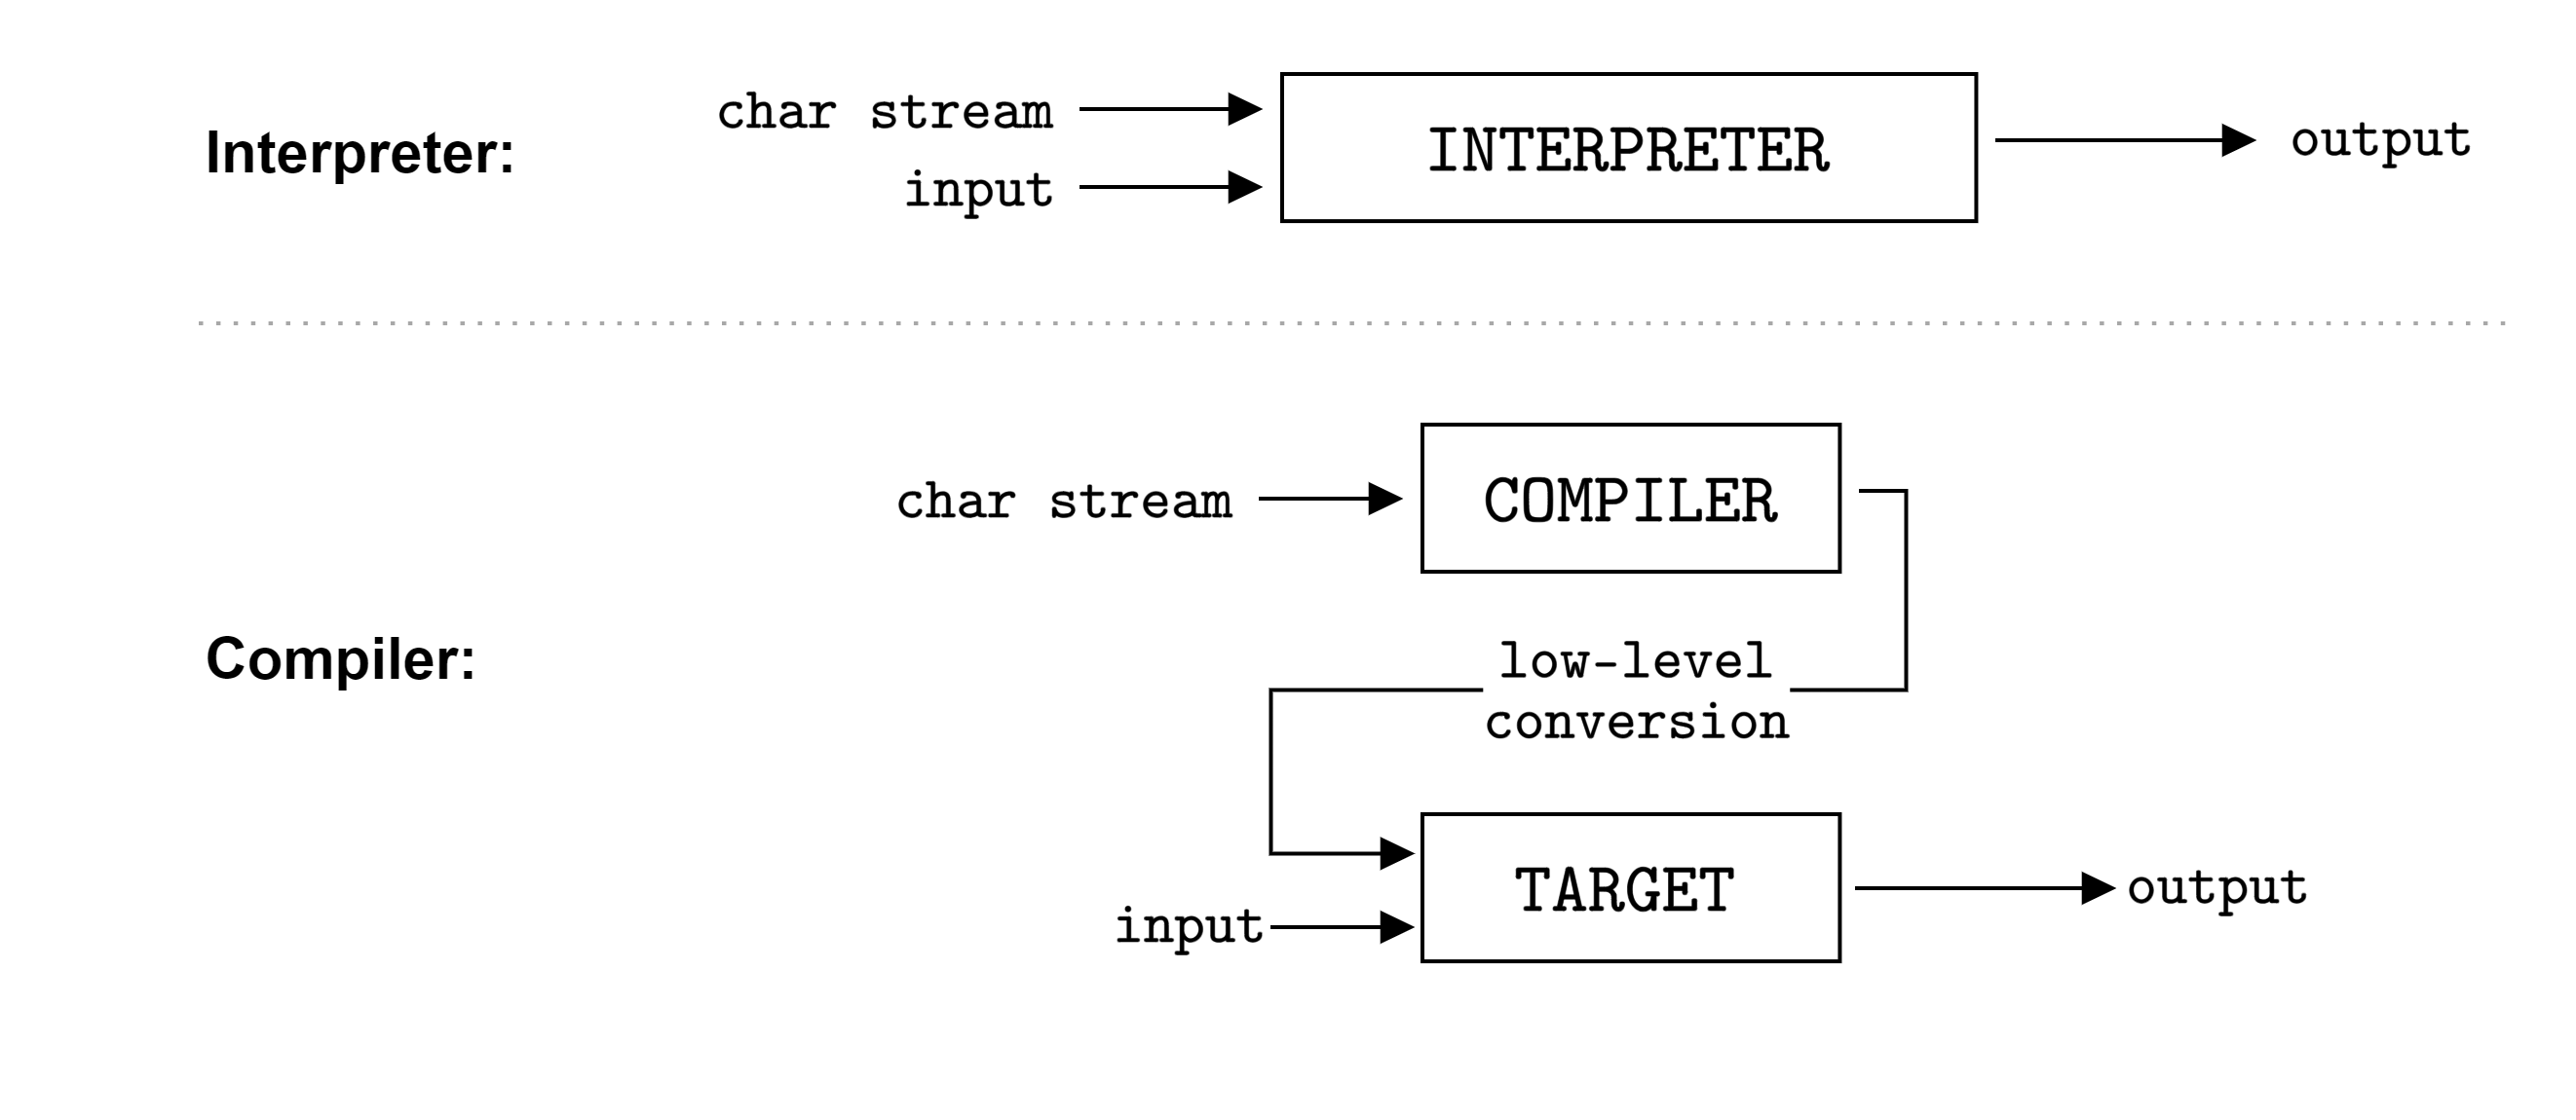
\includegraphics[width=1\textwidth]{Sections/Formal/comp.png}
    \caption{The high-level processes of a compiler and an interpreter.}
\end{figure}

\begin{figure}[h]
    \centering
    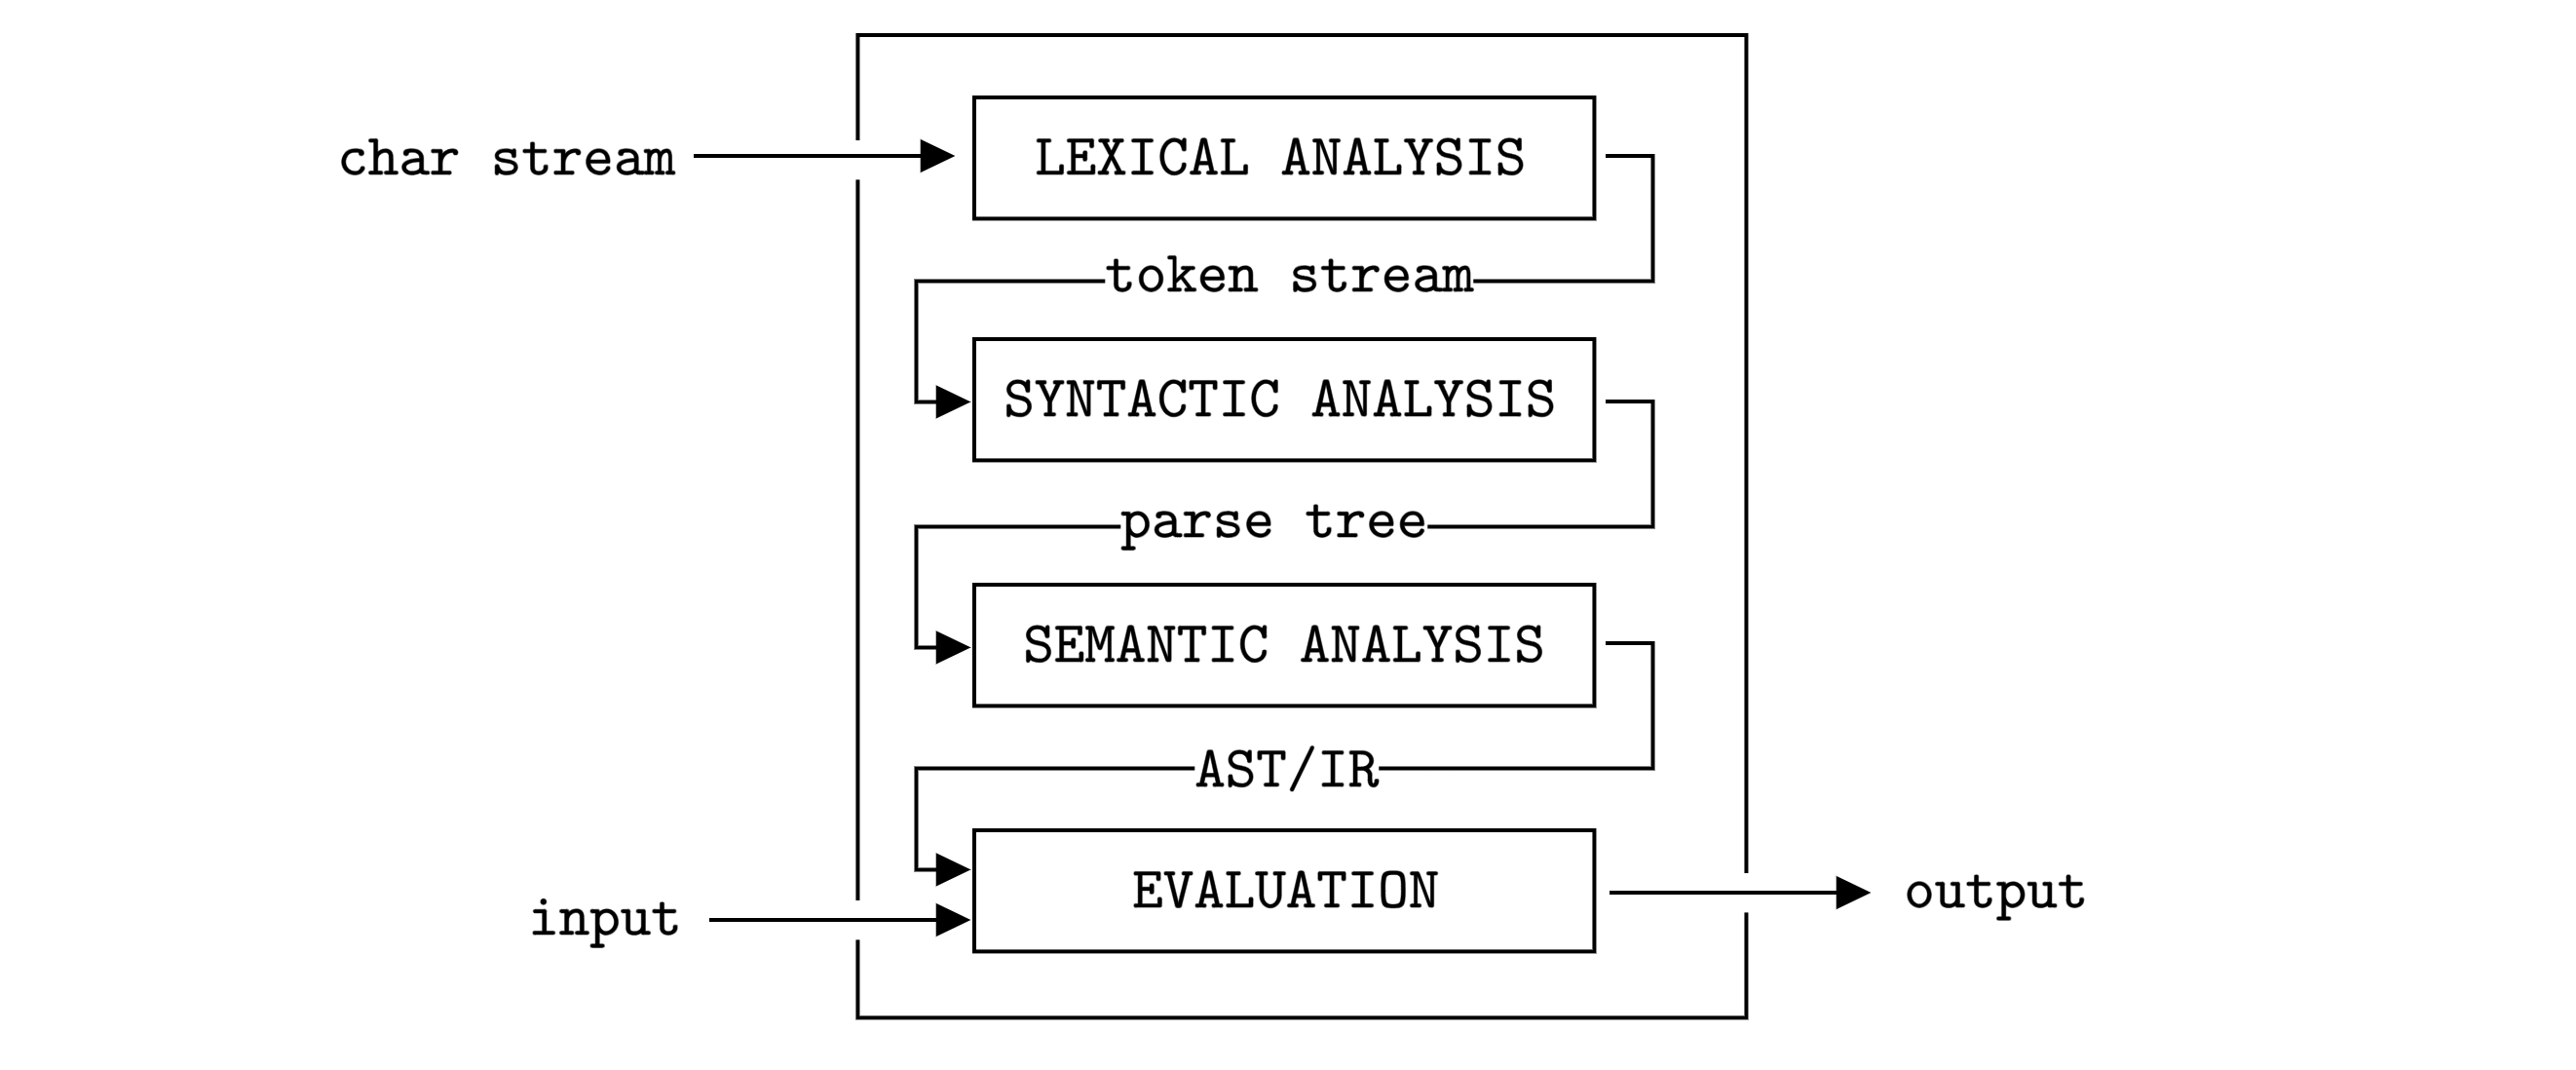
\includegraphics[width=1\textwidth]{Sections/Formal/comp2.png}
    \caption{Stages of program processing: A character stream undergoes lexical, syntactic, and semantic analysis, transforming into an AST or IR before evaluation. Interpreters execute the AST/IR directly, while compilers translate it into machine code.}
\end{figure}

\newpage
    
\noindent
\noindent
To formally layout our language, we use the \textbf{Backus-Naur Form (BNF)} notation. But before we 
do so, we gain some intuition by breaking down an english sentence from its \textbf{terminal symbols} to its \textbf{non-terminal symbols}. Recall these terms from the pre-requisite section (\ref{def:non-terminal-terminal}).\\

\begin{figure}[h]
    \centering
    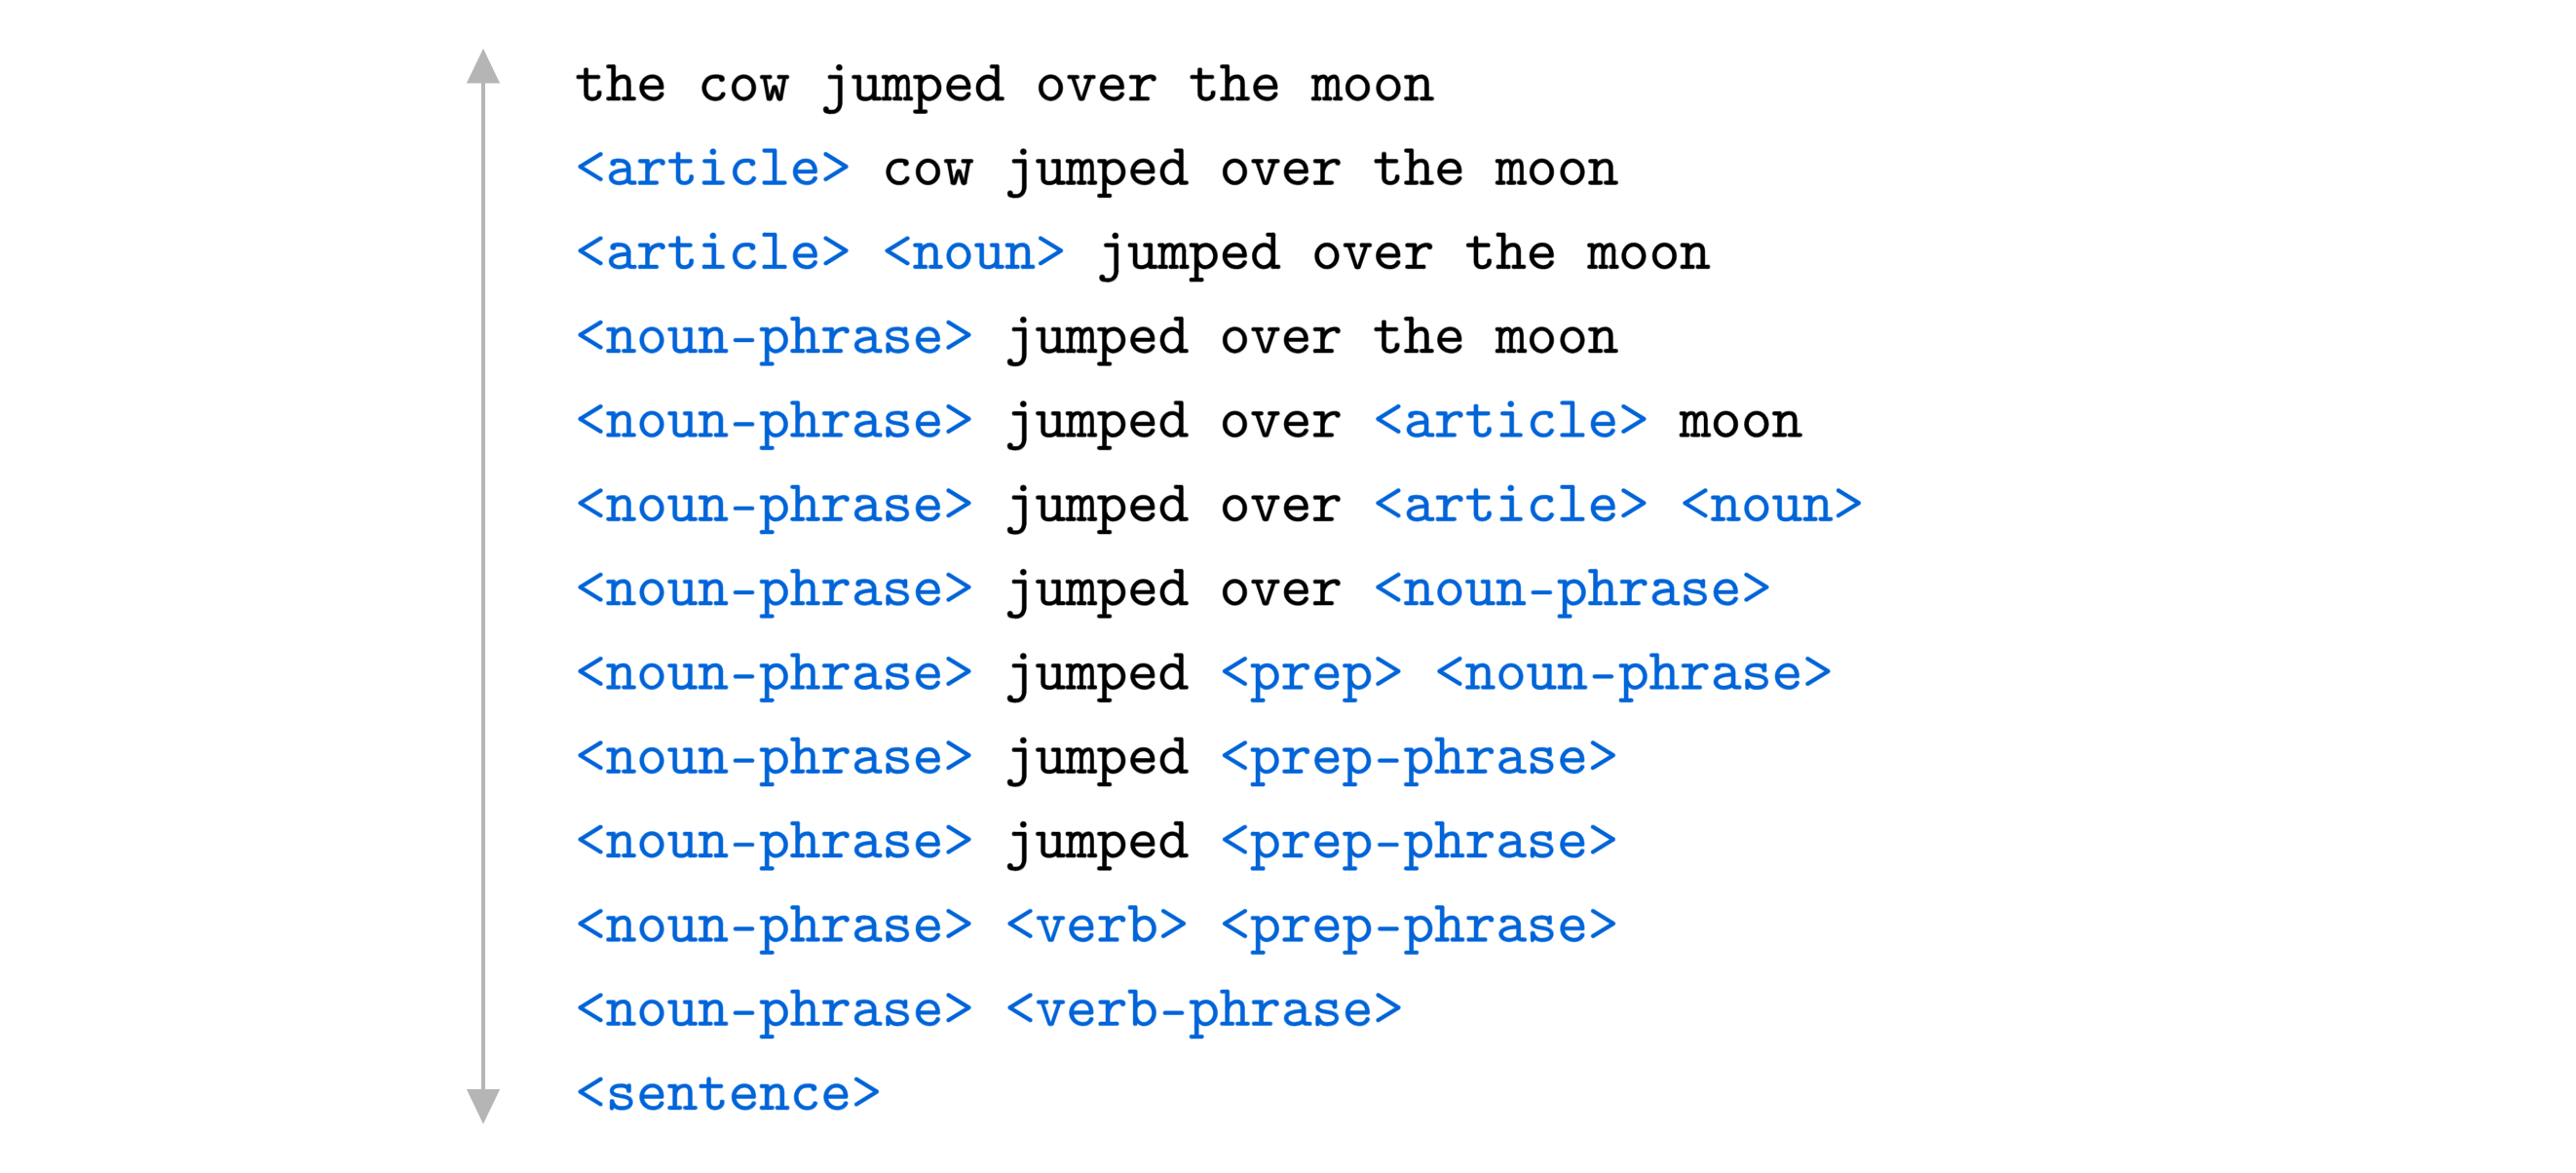
\includegraphics[width=1\textwidth]{Sections/Formal/derivation.png}
    \caption{The sentence ``The cow jumped over the moon.'' broken down into terminal and non-terminal symbols. This is a derivation showing how the sentence is built up from the start symbol of a \texttt{<sentence>}.}
\end{figure}

\noindent
From which the above can be represented in a tree structure:
\begin{figure}[h]
    \centering
    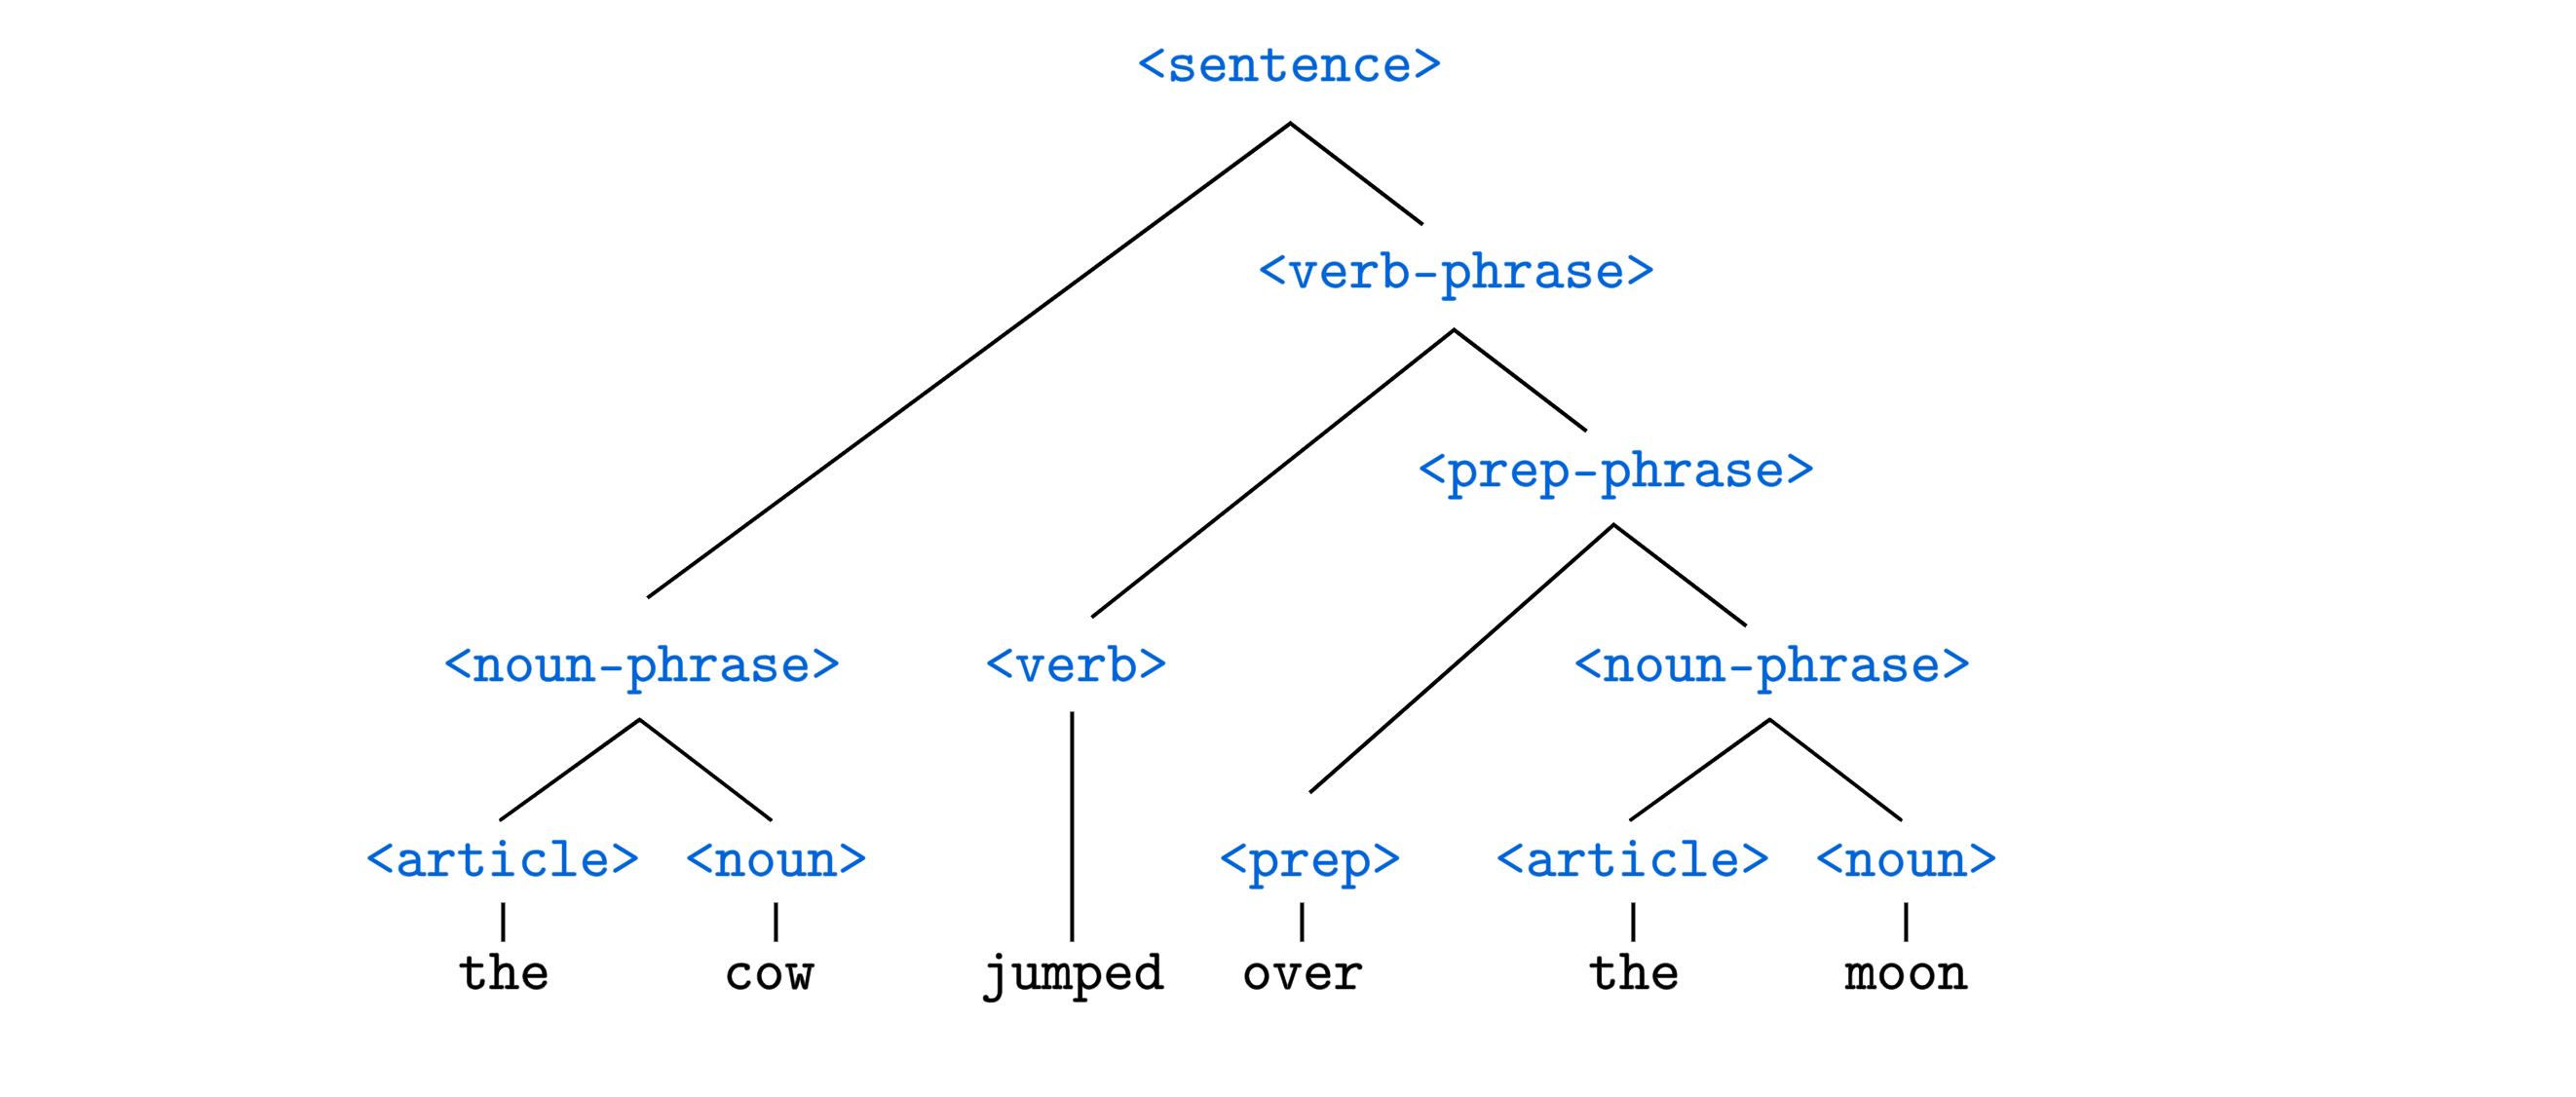
\includegraphics[width=1\textwidth]{Sections/Formal/tree.png}
    \caption{The sentence ``The cow jumped over the moon.'' represented as a \textbf{parse-tree}.}
\end{figure}

\newpage

\noindent
Now if we wanted to state these rules before-hand that a \texttt{<sentence>} is made up of a \texttt{<noun-phrase>} and a \texttt{<verb-phrase>} we can do so as such:

\begin{figure}[h]
    \centering
    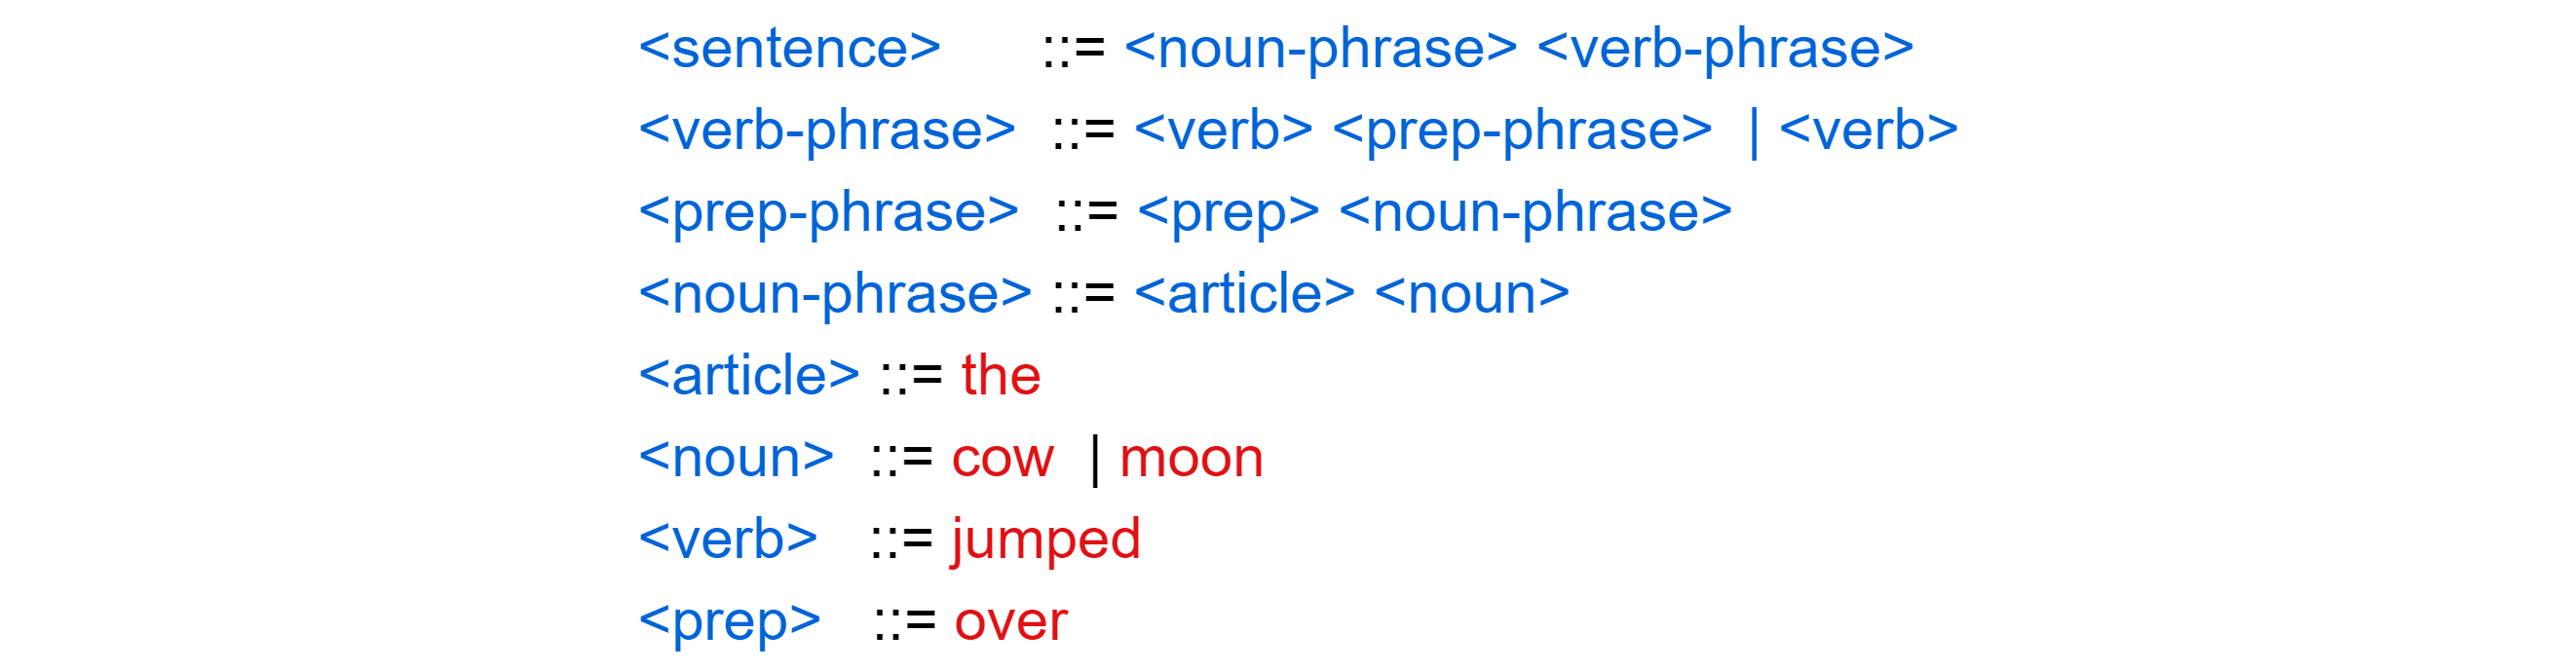
\includegraphics[width=1\textwidth]{Sections/Formal/bnf.png}
    \caption{The rules for the sentence ``The cow jumped over the moon.'' via a thread of production rules (\ref{def:production_rule}). This example illustrates \textbf{Backus-Naur Form (BNF)} notation.}
\end{figure}

\vspace{-1em}
\begin{Def}[Backus-Naur Form (BNF)]

    \textbf{Backus-Naur Form (BNF)} is a formal notation used to define the context. It consists of production rules that specify how symbols in a language can be recursively composed. Each rule follows the form:
    
    \begin{center}
    \texttt{<non-terminal> ::= expression}
    \end{center}
    
    \noindent
    where \texttt{<non-terminal>} represents a syntactic category, and \texttt{expression} consists of terminals, non-terminals, or alternative sequences.
    
    \end{Def}

    \vspace{-.5em}
    \noindent
        Consider a more programmer-like example:

        \begin{figure}[h]
            \centering
            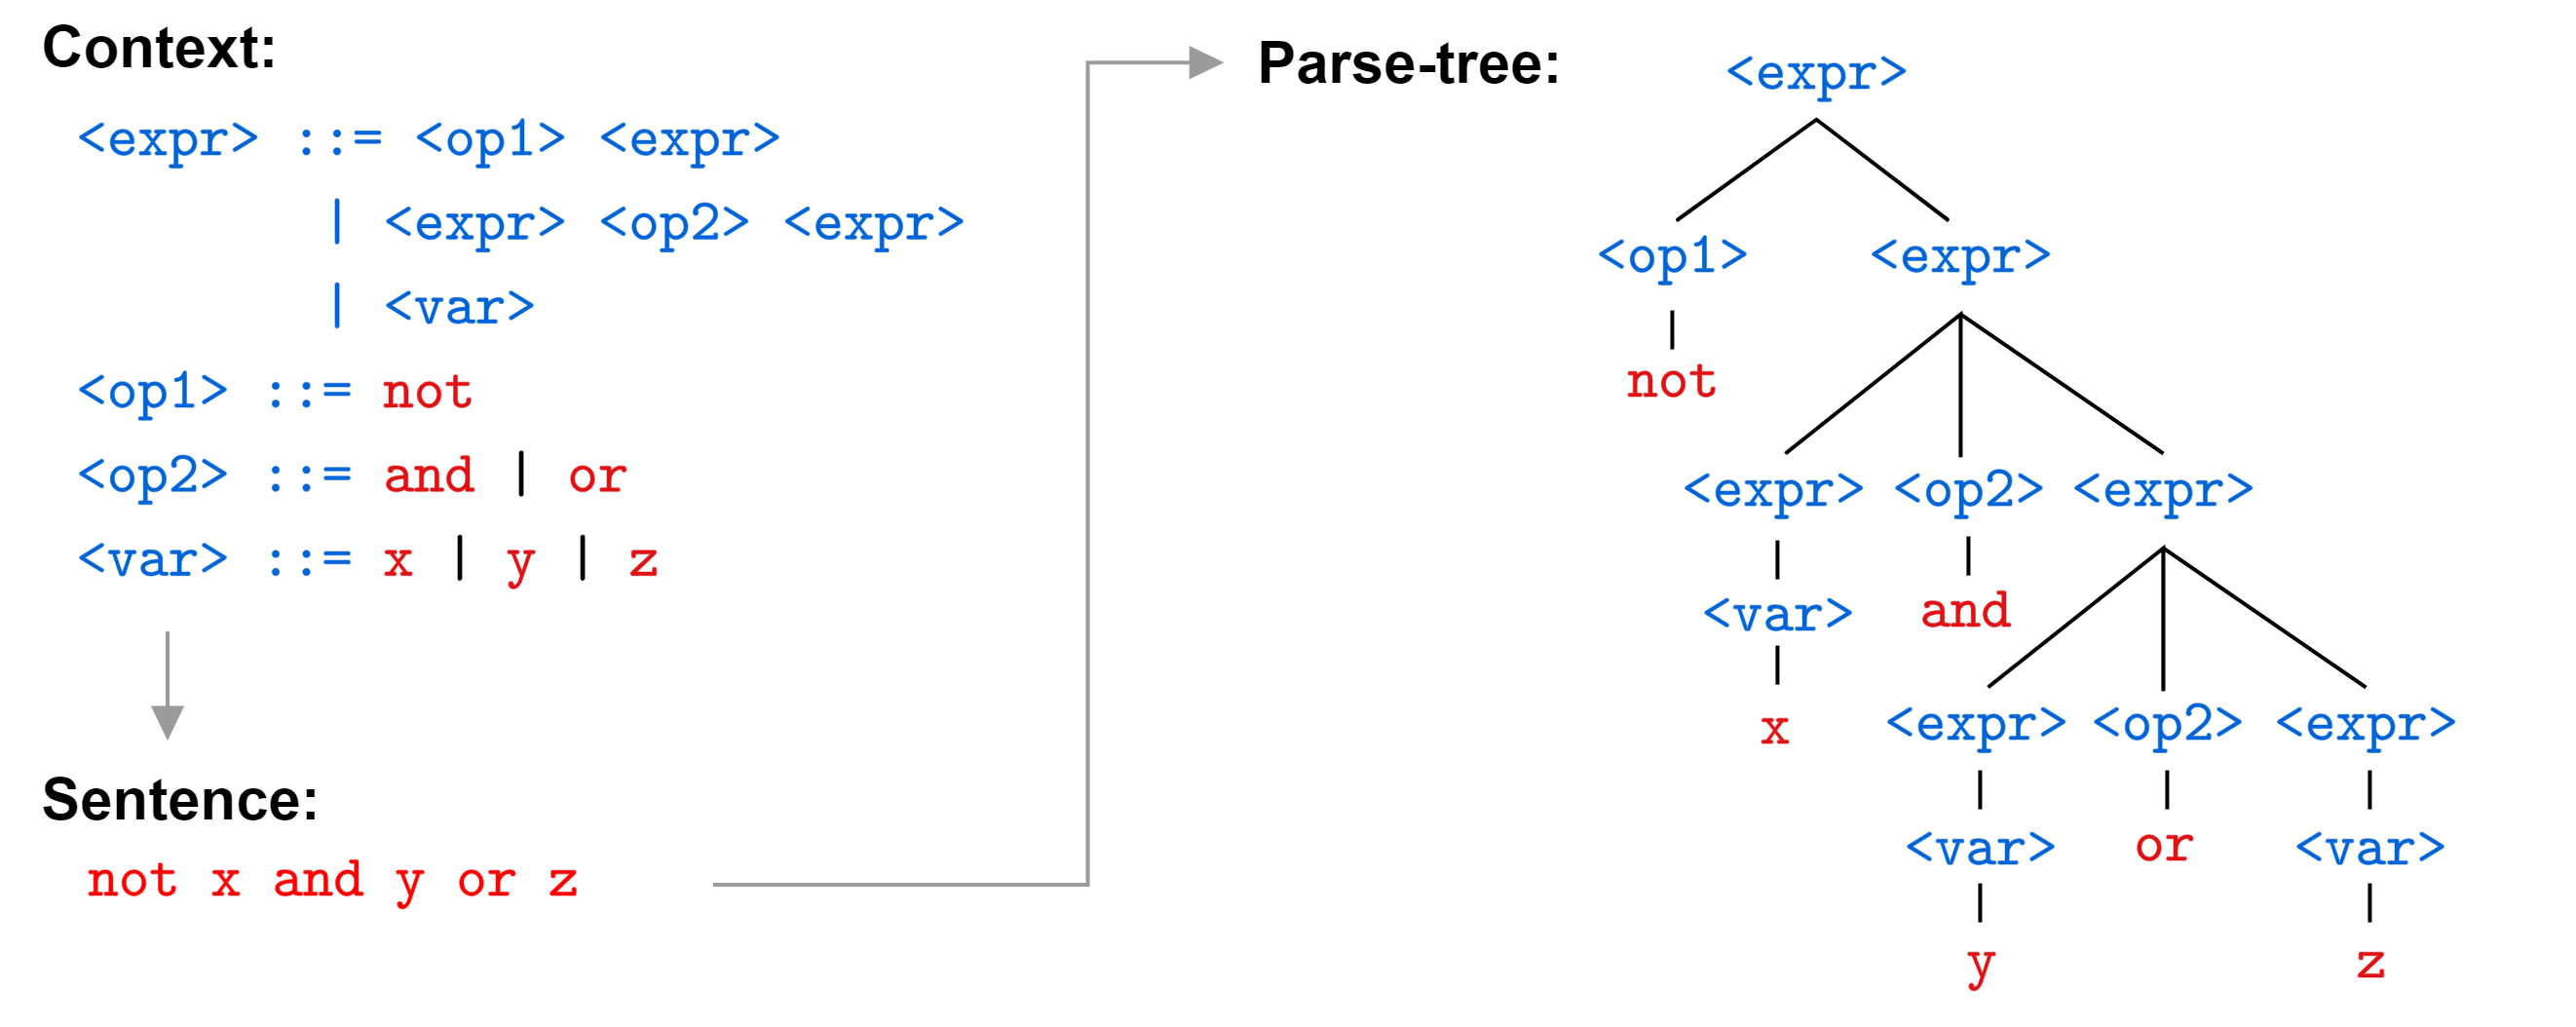
\includegraphics[width=1\textwidth]{Sections/Formal/bnf2.png}
            \caption{A simple language, consisting of \texttt{and} and \texttt{or} operations.}
        \end{figure}

\newpage
